% siminos/atlas/bridge.tex  pdflatex atlas
% $Author$ $Date$

\section{Bridges to nowhere}
\label{s:bridge}

You can safely skip this section, unless you would like to join a brief
tour of the graveyard of obvious ideas and pet symmetry reduction schemes
that all have one thing in common: they do not work.

What follows is very much like the the \refsect{s:cut}; due to the linear
action of the symmetry group, 'slicing' is easier than `sectioning', but
more unfamiliar - that is why we started with reviewing Poincar\'e
sections.

for a history, see remarks in ChaosBook.org

Purely group-theoretical, no dynamics to inform it.

{\bf Polar coordinates}

even for pipe flows one does not use cylindrical Bessel functions
eigenbasis.

{\bf Hilbert bases}

    \DB{2012-04-10}
    {A book report on Hilbert bases by Daniel Borrero}
One approach to symmetry reduction that is often used for low-dimensional
dynamical systems is to rewrite the dynamics in terms of a Hilbert
invariant polynomial basis (see \refref{GL-Gil07b} for a clear and
detailed discussion of this method). The idea here is that one can take
the dynamics in equivariant state space coordinates
$(x_1,x_2,x_3,...,x_d)$ and rewrite them in terms of polynomials of these
variables $(u_1,u_2,u_3,...,u_m)$ that are invariant under the group
action. The algebra required is quite involved and the required
computations become very large for problems with as few as ten
dimensions\rf{gatermannHab}. This makes the method of Hilbert bases
unfeasible for dealing with high-dimensional dynamical systems, such
as turbulent fluid flows.

{\bf Marsdenmania}

Hamiltonian, more complicated

{\bf Method of connections}

example: swimmer

%%%%%%%%%%%%%%%%%%%%%%%%%%%%%%%%%%%%%%%%%%%%%%%%%%%%%%%%%%%%%%%%%%%%%
\begin{figure}
   \centering
  \setlength{\unitlength}{0.20\textwidth}
(a)~~~
  \begin{picture}(1,0.98073806)%
    \put(0,0){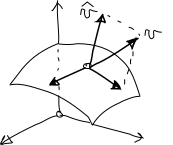
\includegraphics[width=\unitlength]{A28tangents}}%
    \put(0.8635648,0.73622308){\color[rgb]{0,0,0}\makebox(0,0)[lb]{\smash{$\vel$}}}%
    \put(0.49893205,0.86039365){\color[rgb]{0,0,0}\makebox(0,0)[lb]{\smash{$\vel_{\bot}$}}}%
    \put(0.27198728,0.5378933){\color[rgb]{0,0,0}\makebox(0,0)[lb]{\smash{$\groupTan_1$}}}%
    \put(0.58493215,0.33483773){\color[rgb]{0,0,0}\makebox(0,0)[lb]{\smash{$\groupTan_2$}}}%
    \put(0.54959234,0.21257862){\color[rgb]{0,0,0}\makebox(0,0)[lb]{\smash{$\LieEl\ssp$}}}%
  \end{picture}%
(b)~~~
  \begin{picture}(1,0.98655417)%
    \put(0,0){\includegraphics[width=\unitlength]{BeThMconnect}}%
    \put(0.20559239,0.64023845){\color[rgb]{0,0,0}\rotatebox{0.0313674}{\makebox(0,0)[lb]{\smash{$\ssp(\zeit)$}}}}%
    \put(0.68383186,0.20519203){\color[rgb]{0,0,0}\rotatebox{0.0313674}{\makebox(0,0)[lb]{\smash{$\ssp(0)$}}}}%
    \put(0.67475925,0.8109461){\color[rgb]{0,0,0}\rotatebox{0.0313674}{\makebox(0,0)[lb]{\smash{$\sspRed(\zeit)$}}}}%
    \put(0.35760559,0.8662057){\color[rgb]{0,0,0}\rotatebox{0.0313674}{\makebox(0,0)[lb]{\smash{$\LieEl(\zeit)$}}}}%
    \put(0.70884327,0.61850672){\color[rgb]{0,0,0}\rotatebox{0.0313674}{\makebox(0,0)[lb]{\smash{$\vel_{\bot}$}}}}%
  \end{picture}%
   \caption{\label{fig:BeThMconnect}
    (a)
By equivariance $\vel(\ssp)$ can be replaced by $\vel_\bot(\ssp)$, the
velocity normal to the group tangent directions at \statesp\ point $\ssp$.
    (b)
Method of connections replaces $\vel(\sspRed)$ at every instant
$\sspRed =\sspRed(\zeit)$ by $\vel_\bot(\sspRed)$, so in
$\sspRed(\zeit)$ co-moving frame there is no motion along the group
tangent directions.
}
\end{figure}
%%%%%%%%%%%%%%%%%%%%%%%%%%%%%%%%%%%%%%%%%%%%%%%%%%%%%%%%%%%%%%%%%%%%%

    \ifdraft\color{blue}
    \begin{itemize}
      \item refer to \reffig{fig:BeThMconnect}
      \item gauge fixing, geometric phase?
    \end{itemize}
    \color{black}\fi


{\bf A co-moving frame}
Visualizing a single `relative' trajectory in its co-moving frame, moving with
the mean {\phaseVel} of a given solution, is useful if we are
concerned with that individual solution.
    \PC{cite Golubitsky}
A co-moving frame is useless if
we are concerned with studying collections of these trajectories, as each
solution travels with its own mean {\phaseVel}, and there is no single
co-moving frame that can simultaneously reduce \emph{all} traveling
solutions.
    \PC{disparage co-moving frames: they are misleading for \rpo s, as they
    misrepresent time segments for which a \po\ might be glued to
    barely unstable \eqv. A co-moving frame rotates with the constant
    mean
    $\timeAver{\velRel}= \shift_p/\period{p}
    \,.
    $ We \emph{emphatically} do not work in
    co-moving frames.}
    \PC{unhappy about ``moving frames'': misleading, as slice is
     \emph{emphatically} stationary. ''Covariant frames'' move, but we
     do not know how to use them
     }
